\documentclass{beamer}

\usepackage[T1]{fontenc}
\usepackage[utf8]{inputenc}
\usepackage[slovene]{babel}
\usepackage{etoolbox}
\usepackage{algorithm2e}
\usepackage{listings}


\mode<presentation>
{
  \usetheme{default}
  \setbeamercovered{transparent}
}

\makeatletter
\appto\verbatim@font{\footnotesize}
\makeatother

\setbeamertemplate{navigation symbols}{}

\newcommand{\bx}{\mathbf{x}}
\DeclareMathOperator{\Gl}{Gl}
\DeclareMathOperator{\adj}{adj}
\newtheorem{proposition}[theorem]{Proposition}

\title[Paralelizacija grafovskih algoritmov v funkcijskih jezikih]
{Paralelizacija grafovskih algoritmov v funkcijskih jezikih}

\author[Avtor: Tjaž Eržen, Mentor: doc. dr. Matija Pretnar]
{Avtor: Tjaž Eržen\\Mentor: doc. dr. Matija Pretnar}

\date[24. april 2024]
{Dolga predstavitev pri Diplomskem seminarju, 24. april 2024}

\lstdefinelanguage{OCaml}{
  keywords={let,rec,if,then,else,module},
  sensitive=true,
  basicstyle=\ttfamily,
  keywordstyle=\bfseries,
  showstringspaces=false,
  morecomment=[s]{(*}{*)},
  morestring=[b]"
}

\lstset{
  language=Caml,
  frame=single,
  numbers=left,
  numberstyle=\tiny,
  stepnumber=1,
  numbersep=5pt,
  tabsize=2,
  breaklines=true,
  prebreak=\raisebox{0ex}[0ex][0ex]{\ensuremath{\hookleftarrow}},
  showtabs=false,
  showspaces=false,
  showstringspaces=false,
  basicstyle=\ttfamily\small,
  identifierstyle=\ttfamily\small,
  commentstyle=\color{gray}\ttfamily\small,
  keywordstyle=\color{blue}\ttfamily\small,
  stringstyle=\color{red}\ttfamily\small
}

\begin{document}

\section{Uvod}

\begin{frame}
  \titlepage
\end{frame}

\begin{frame}
  \tableofcontents
\end{frame}

% Uvod: Povej da si raziskoval, kako pohitriti grafovske algoritme s pomocjo paralelizacije.
% Implementirali bomo paralelne razlicice algoritmov, kot so BFS, Dijkstra, Floyd-Warshall.
% Uporabili bomo Domainslib, ki je knjiznica za paralelno programiranje v OCamlu.

\begin{frame}{Uvod}
    \begin{itemize}
        \item Paralelizacija v funkcijskih jezikih
        \item Domainslib
        \item Sistemi s skupnim pomnilnikom
        \item Dirka podatkov
    \end{itemize}
\end{frame}

\begin{frame}{Uvod}
  \begin{figure}
    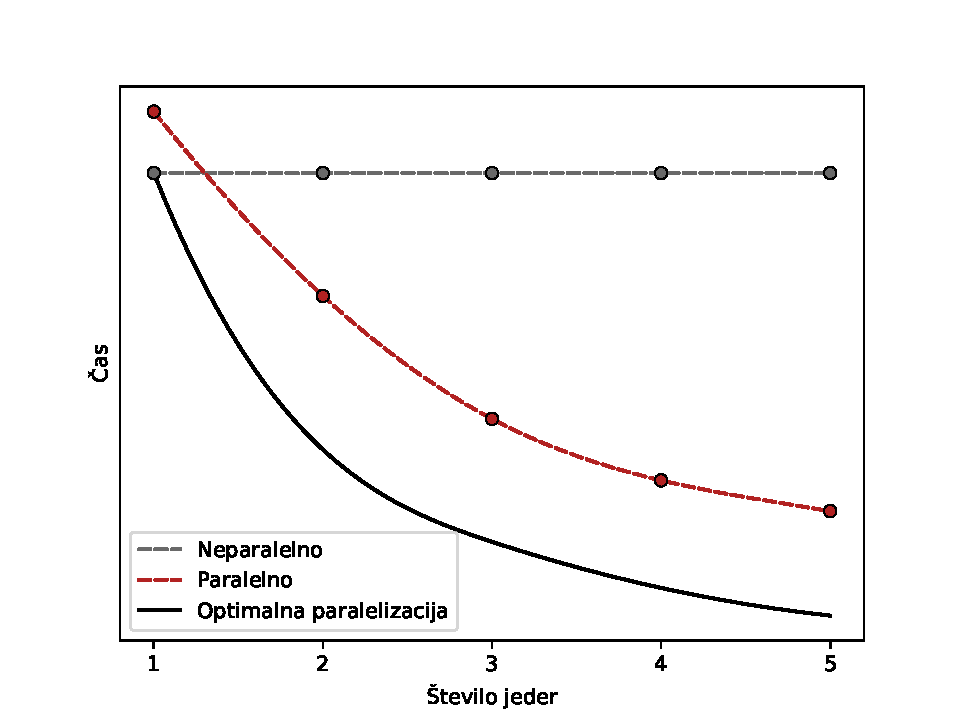
\includegraphics[width=6cm]{slike/cilj-casovne-zahtevnosti-paralelizacije.pdf}
  \end{figure}
\end{frame}

\section{Paralelno računanje Fibonaccijevih števil}

\begin{frame}[fragile]
  \frametitle{Paralelni izračun Fibonaccijevih števil}
  \begin{itemize}
    \item Fibonaccijeva števila: $F_0 = 0, F_1 = 1, F_n = F_{n-1} + F_{n-2}$
    \item Optimizacija: Paralelno računanje $F_{n-1}$ in $F_{n-2}$
    \item Prag sekvenčnosti
  \end{itemize}
  \begin{verbatim}
  module T = Domainslib.Task

  let rec fib n = 
    if n < 2 then 1 else fib (n - 1) + fib (n - 2)
  
  let rec fib_par pool n =
    if n <= 38 then fib n
    else
      let a = T.async pool (fun _ -> fib_par pool (n - 1)) in
      let b = T.async pool (fun _ -> fib_par pool (n - 2)) in
      T.await pool a + T.await pool b
  \end{verbatim}
\end{frame}

\begin{frame}
  \frametitle{Čas izračuna Fibonaccijevega števila v odvisnosti od števila domen}
  \begin{figure}[h!]
    \centering
    % \caption{Čas izračuna 43. Fibonaccijevega števila v odvisnosti od števila domen}
    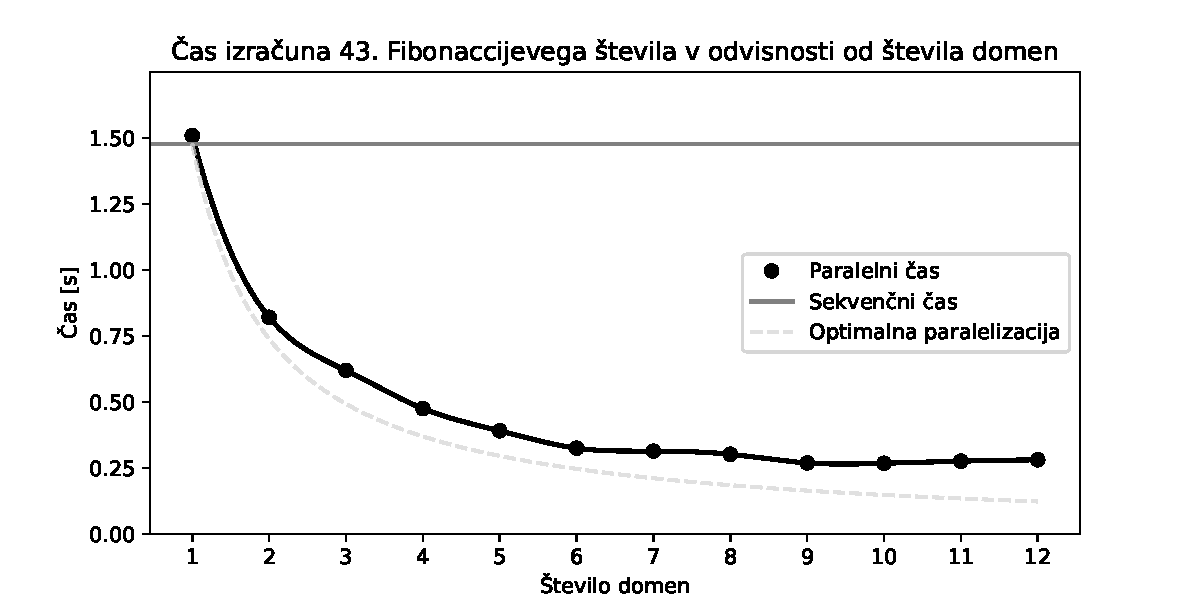
\includegraphics[width=10cm]{slike/fib_par_v_odvisnosti_od_domen.pdf}
  \end{figure}
\end{frame}

\begin{frame}
  \frametitle{Čas izračuna Fibonaccijevega števila v odvisnosti od $n$}
  \begin{figure}[h!]
    \centering
    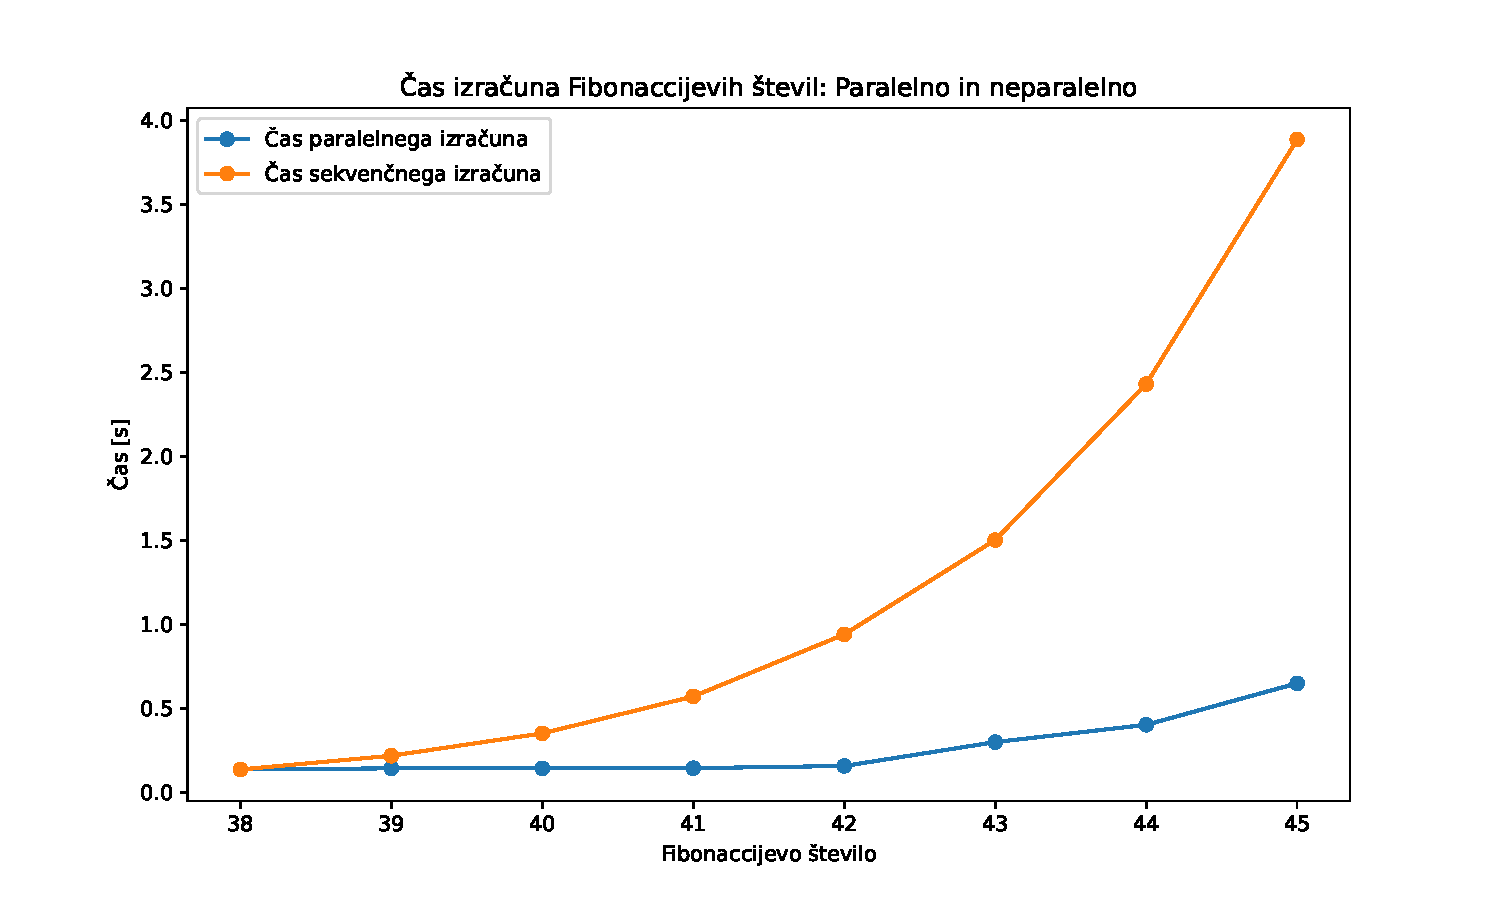
\includegraphics[width=10cm]{slike/fib_par_v_odvisnosti_od_n.pdf}
  \end{figure}
\end{frame}

\section{Predstavitev grafa v funkcijskih jezikih}

\begin{frame}[fragile]
  \frametitle{Predstavitev vozlišča}
  \begin{verbatim}
  module Node : sig
    type t
    val compare : t -> t -> int
    val create : int -> t
    val value : t -> int
    val to_string : t -> string
  end = struct
    type t = { id : int; value : int }
  
    let compare node1 node2 = 
      Stdlib.compare node1.id node2.id
    ...
  end
  module NodeSet = Set.Make (Node)
  module NodeMap = Map.Make (Node)
  \end{verbatim}
\end{frame}

\begin{frame}[fragile]
  \frametitle{Predstavitev neuteženega grafa}
  \begin{verbatim}
    module UnweightedGraph : sig
    type t
  
    val empty : directed:bool -> t
    val add_node : Node.t -> t -> t
    val remove_node : Node.t -> t -> t
    val add_edge : Node.t -> Node.t -> t -> t
    val remove_edge : Node.t -> Node.t -> t -> t
    val nodes : t -> Node.t list
    val edges : t -> (Node.t * Node.t) list
    val to_string : t -> string
    val neighbours : Node.t -> t -> Node.t list
  end = struct
    type t = {
      edges : NodeSet.t NodeMap.t;
      directed : bool;
    }
    ...
  end  
  \end{verbatim}
\end{frame}

\section{Paralelno iskanje v širino}

% \begin{frame}
  \frametitle{Iskanje v širino}
  \begin{frame}
    \frametitle{BFS algoritem}
    \begin{figure}[h!]
      \centering
      \includegraphics[width=10cm]{slike/bfs-algorithm-visualization.pdf}
    \end{figure}
  \end{frame}
% \end{frame}

\begin{frame}[fragile]
  \frametitle{Paralelno iskanje v širino}
  % \begin{itemize}
  %   \item Sekvenčno: Vozlišča raziskuj v vrsti (FIFO)
  %   \item Paralelno: Vozlišča raziskuj v množici po nivojih
  % \end{itemize}

  \begin{verbatim}
  let rec loop_inner visited stages mapper graph =
    match stages with
    | last_stage :: _ ->
        let all_neighbors =
          last_stage |> NodeSet.elements |> mapper
          |> List.fold_left NodeSet.union NodeSet.empty
        in
        let next =
          NodeSet.diff all_neighbors visited
          |> NodeSet.elements
          |> List.fold_left
              (fun set node -> NodeSet.add node set)
              NodeSet.empty
        in
        if NodeSet.is_empty next then List.rev stages
        else
          loop_inner
            (NodeSet.union visited next)
            (next :: stages) mapper graph
    | [] -> failwith "Should not happen"

  \end{verbatim}
\end{frame}

\begin{frame}[fragile]
  \frametitle{Paralelno iskanje v širino}

\begin{itemize}
  \item Sekvenčno
  \begin{verbatim}
let mapper_seq = fun nodes -> 
  nodes |> List.map (
    fun node -> UnweightedGraph.neighbours node graph)
  \end{verbatim}
  \item Paralelno
  \begin{verbatim}
module T = Domainslib.Task
let parallel_map f task_pool arr =
  let len = Array.length arr in
  let res = Array.make len (f arr.(0)) in
  T.parallel_for task_pool start:0 finish:(len - 1) 
    body:(fun i -> res.(i) <- f arr.(i));
  res
in
let mapper = fun nodes ->
  nodes |> Array.of_list |> parallel_map (
    fun node -> UnweightedGraph.neighbours node graph) task_pool
  \end{verbatim}
\end{itemize}
  
\end{frame}


\end{document}
